\documentclass[modern, letterpaper]{aastex61}
% \documentclass[twocolumn]{aastex61}

% to-do list
% ----------
% - Add items here.

% style notes
% -----------
% - This file generates by Makefile; don't be typing ``pdflatex'' or some bullshit.
% - Line break between sentences to make the git diffs readable.
% - Use \, as a multiply operator.
% - Reserve () for function arguments; use [] or {} for outer shit.
% - Use \sectionname not Section, \figname not Figure, \documentname not Article or Paper or paper.
% - Use "comoving" instead of "co-moving".
% - Write elements as \elem{X}.

% packages
\definecolor{cbblue}{HTML}{3182bd}
\usepackage{microtype}  % ALWAYS!
\usepackage{amsmath,amssymb,natbib}
\usepackage[flushleft]{threeparttable}
\hypersetup{backref,breaklinks,colorlinks,urlcolor=cbblue,linkcolor=cbblue,citecolor=black}
\graphicspath{{figures/}}
\bibliographystyle{aasjournal}

% define macros for text
\newcommand{\project}[1]{\textsl{#1}}
\newcommand{\acronym}[1]{{\small{#1}}}
\newcommand{\gaia}{\project{Gaia}}
\newcommand{\rave}{\project{\acronym{RAVE}}}
\newcommand{\apogee}{\project{\acronym{APOGEE}}}
\newcommand{\tmass}{\project{\acronym{2MASS}}}
\newcommand{\documentname}{Article}
\newcommand{\sectionname}{Section}
\newcommand{\figname}{Figure}
\newcommand{\eqname}{Equation}
\newcommand{\dr}{\acronym{DR1}}
\newcommand{\tgas}{\acronym{TGAS}}
\newcommand{\etal}{\textit{et al}.}
\newcommand*\elem[1]{\ensuremath{\mathrm{#1}}}
\newcommand*\elemH[1]{\ensuremath{[\mathrm{#1}/\elem{H}]}}
\newcommand*\teff{\ensuremath{T_\mathrm{eff}}}
\newcommand*\logg{\ensuremath{\log{g}}}
\newcommand*{\feh}{\ensuremath{\elemH{Fe}}}
\newcommand{\sunanalog}{\text{Krios}}
\newcommand{\bizarreone}{\text{Kronos}}
\newcommand{\Tcondens}{\ensuremath{T_C}}
\newcommand{\mearth}{\ensuremath{M_\oplus}}
\newcommand{\mjupiter}{\ensuremath{M_\mathrm{Jup}}}

% define macros for math
\newcommand{\given}{\,|\,}
\newcommand{\normal}{{\mathcal{N}}}
\newcommand{\dd}{\mathrm{d}}
\newcommand{\transp}[1]{{#1}^{\!\mathsf{T}}}
\newcommand{\inv}[1]{{#1}^{-1}}
\newcommand{\bs}[1]{\boldsymbol{#1}}
\newcommand{\vperp}{\bs{v}^\perp}
\newcommand{\propm}{\bs{\mu}}
\newcommand{\mat}[1]{\mathbf{#1}}
\renewcommand{\vec}[1]{\bs{#1}}
\newcommand{\kms}{\ensuremath{\rm km~s^{-1}}}
\newcommand{\msun}{{\rm M}_\odot}
\newcommand{\pc}{{\rm pc}}
\newcommand{\data}{\mathrm{data}}
\newcommand{\snr}{[S/N]_\varpi}
\newcommand{\eye}{\mathbb{I}}
\newcommand{\absdvtan}{\ensuremath{|\Delta\vec v_\mathrm{t}|}}
\newcommand{\estimates}{\ensuremath{\{\hat{\varpi_i},\hat{\mu_{\alpha,i}},\hat{\mu_{\delta,i}},\hat{v_{r,i}}\}}}

\newcommand{\todo}[1]{{\color{blue}TODO:#1}}

\renewcommand\tablename{Table}

\begin{document}\sloppy\sloppypar\raggedbottom\frenchspacing % trust me

\title{
  Kronos \& Krios:
  Evidence for accretion of massive, rocky planetary system in a sun-like pair
}

\author[0000-0001-7790-5308]{Semyeong Oh}
\affil{Department of Astrophysical Sciences, Princeton University, 4 Ivy Lane, Princeton, NJ 08544, USA}
\affil{To whom correspondence should be addressed: \texttt{semyeong@astro.princeton.edu}}

\author[0000-0003-0872-7098]{Adrian M. Price-Whelan}
\affil{Department of Astrophysical Sciences, Princeton University, 4 Ivy Lane, Princeton, NJ 08544, USA}

\author{John M. Brewer} % TODO: need ORCID
\affil{Department of Astronomy, Yale University, 260 Whitney Ave, New Haven, CT 06511, USA}

\author[0000-0003-2866-9403]{David W. Hogg}
\affil{Center for Computational Astrophysics, Flatiron Institute, 162 Fifth Ave, New York, NY 10010, USA}
\affil{Center for Cosmology and Particle Physics, Department of Physics, New York University, 726 Broadway, room 1005, New York, NY 10003, USA}
\affil{Center for Data Science, New York University, 60 Fifth Ave, New York, NY 10011, USA}
\affil{Max-Planck-Institut f\"ur Astronomie, K\"onigstuhl 17, D-69117 Heidelberg}

\author{David N. Spergel} % TODO: need ORCID
\affil{Center for Computational Astrophysics, Flatiron Institute, 162 Fifth Ave, New York, NY 10010, USA}

% \author{Keith A. Hawkins}
% \affil{Department of Astronomy, Columbia University, 550 W 120th St, New York, NY 10027, USA}

% \author{Nathan W. C. Leigh}
% \affil{Department of Astrophysics, American Museum of Natural History, Central Park West and 79th St, New York, NY 10024, USA}

\author{Justin Myles} % TODO: need ORCID
\affil{Department of Astronomy, Yale University, 260 Whitney Ave, New Haven, CT 06511, USA}

\begin{abstract}
  We report and discuss the discovery of a comoving pair of bright solar-type
  stars, HD~240430 and HD~240429, with a significant difference in their
  chemical abundances.
  The two stars have an estimated separation of $\approx 0.6$~pc at a distance of
  $r\approx 100~\pc$ with nearly identical three-dimensional velocities,
  %($|\Delta \bs{v}| < XX~\kms$ with 95\% confidence),
  as inferred from \gaia\ \tgas\ parallaxes and proper motions, and
  high-resolution radial velocity measurements.
  Stellar parameters determined from high-resolution Keck HIRES spectra
  indicate that both stars are $\sim 4$~Gyr old,
  yet both stars show high surface \elem{Li} abundance for this age.
  The more metal-rich of the two, HD~240430, shows an enhancement of
  refractory ($\Tcondens>1200$~K) elements by $\approx 0.2$~dex but not as
  large enhancement of (moderately) volatile elements ($\Tcondens<1200$~K; \elem{C},
  \elem{N}, \elem{O}, \elem{Na}, and \elem{Mn}):
  this is the largest and the most significant difference found in
  wide binary pairs yet.
  The proximity in phase space and ages between the two stars suggests that
  they formed together with the same composition, at odds with the observed
  differences in metallicity and abundance patterns.
  We therefore suggest that the star HD~240430, ``Kronos'', recently accreted $\approx 20$~\mearth\ of
  rocky material after birth selectively enhancing the refractory elements in
  its surface and convective envelope.
  The other star HD~240429, ``Krios'', may also have had a similar accretion event given
  its high surface \elem{Li} abundance but of much smaller amount
  ($\approx 4$~\mearth).
  Follow-ups to study the existence and properties of the planetary systems
  around these stars will help illuminate more on planet-star interactions.
\end{abstract}

\keywords{
  binaries: visual
  ---
  planet-star interactions
  ---
  stars: abundances
  ---
  stars: formation
  ---
  stars: individual (HD~240430, HD~240429)
  ---
  stars: solar-type
}

\section{Introduction} % (fold)
\label{sec:introduction}

Wide binary stars are valuable tools for studying star and planet formation as well
as Galactic dynamics and chemical evolution.
In the context of studying the evolution of the Milky Way, they are useful for
two main reasons.
First, because wide binaries are weakly bound systems that may be tidally
disrupted by, e.g., field stars, molecular clouds, or the Galactic tidal field,
their statistics can be informative of the Galactic mass distribution.
For example, the separation distribution of halo binaries has been used to
constrain the mass of massive compact halo objects (\citealt{Yoo:2004aa}).
On the other hand, they are also prime targets to test the chemical tagging
hypothesis that stars from the same birthplace may be traced back using detailed
chemical abundance patterns as birth ``tag''s (\citealt{2002ARA&A..40..487F}).
A multiple-star system of any size that we believe are born together can serve
this purpose, with massive open clusters at one extreme.
Wide binaries are at the other extreme in that we may be less confident of the
coevality of individual systems but they are much more abundant than larger
systems like open clusters, rendering their statistics a meaningful indication
of whether the hypothesis works.

Wide binaries with similar or very different planetary architectures around the
component stars have been used to connect a host star's chemistry to its
planetary system.
A differential analysis may reveal chemical signatures related to planet
formation or accretion without any regard to Galactic chemical evolution as
long as the two stars are assumed to be born together with identical
composition.
For close-in giant planets, it has been established that the planet-metallicity
relation is primordial, and that the enhanced metallicity in giant
planet-hosting stars likely promotes the formation of giant planets by
increasing the availability of small particle condensates that form
planetesimals (\citealt{Fischer:2005aa}).
On the other hand, if host stars are polluted after their birth by rocky
planetary material with high refractory-to-volatile ratio, the convective
envelope of the stars may be enhanced in refractory elements (e.g., \elem{Fe})
compared to their initial state.
Thus, differences in planet formation or accretion in two otherwise identical
stars may imprint differences in chemical abundances that depend on the
condensation temperature (\Tcondens).
Several systems in which at least one star hosts at least one planet
have been studied so far with high resolution spectroscopy in this context
(\citealt{Teske:2013aa,Mack:2014aa,Liu:2014aa,Teske:2015aa,Saffe:2015aa,
  Ramirez:2015aa,Biazzo:2015aa,Mack:2016aa,Teske:2016aa,Teske:2016ab}).
The results and interpretations of these studies are varied:
while some systems appear to have undetectable differences
(see also \citealt{Desidera:2004aa,Gratton:2001aa}), other
studies have reported a \Tcondens-dependent difference in abundance
with higher-\Tcondens\ elements showing larger differences.
The increasing abundance difference with condensation temperature has been
attributed both to more yet-undiscovered rocky planets around the relatively
refractory-poor star and to late time accretion of refractory-rich planetary
material (\citealt{Ramirez:2015aa,Biazzo:2015aa}).
The observed differences are $\lesssim 0.1$~dex even in the most dramatic case,
and often at $\approx 0.05$~dex level making them challenging to detect even
with a careful analysis of high-resolution high signal-to-noise ratio spectra.
% maybe want to point out the former interpretation roots back to melendez+09
% and some doubt to that interpretation...

So far the strongest evidence for accretion of planetary material by a host
star comes from spectral analysis of polluted white dwarfs (WDs).
Because the gravitational settling times of elements heavier than \elem{He} in
atmosphere is much shorter than the WD cooling time, detection of metals likely
indicates the presence of a reservoir of dusty material around the WD.
Indeed, many of the polluted WDs host a dusty debris disk detected
in the infrared.
Some of the most dramatically polluted WDs show
surface abundances closely matched by rocky planetary material
with, e.g., bulk Earth composition, strongly arguing
that the disk formed from tidally disrupted minor planets
(\citealt{Zuckerman:2007aa,Klein:2010aa}).
Recently, transit signals from small bodies orbiting around a polluted WD
have been detected by \project{Kepler} adding further support to the picture
(\citealt{2015Natur.526..546V}).

Here, we report and discuss the discovery of a comoving pair of solar twin stars,
HD~240430 and HD~240429, with unusual chemical abundance and differential abundance patterns
that strongly suggest dramatic accretion of planetary material by the two stars.
We nickname the two stars \bizarreone\ (HD~240430) and
\sunanalog\ (HD~240429) throughout the \documentname.
In \sectionname~\ref{sec:data} we present the astrometric and spectroscopic data
about the two stars relevant to the present discussion.
In \sectionname~\ref{sec:discussion} we discuss possible interpretations of
the abundance difference between the pair.
We summarize our discussions in \sectionname~\ref{sec:summary}.

Throughout the \documentname\, we use the following convention for
chemical abundances of stars: \elemH{X} is the ratio of number density of
element \elem{X} to \elem{H} relative to the solar value.
The absolute abundance of \elem{X} is
$A(\elem{X}) = \log_{10} (n_\elem{X}/n_\elem{H})$
where $n_\elem{X}$ is the number density of element \elem{X}.

\subsection{Review of Detailed Chemical Abundance Studies of Wide Binary Stars}
\label{sub:review}

Anticipating the forthcoming discussion, we review and summarize a handful of
wide binary systems that have been studied in
their detailed chemical abundances so far with high-resolution spectroscopy.
These systems are HD~20782/HD~20781, HD~80606/HD~80607, XO-2N/XO-2S, HAT-P-1,
WASP-94A/WASP94-B, and HD~133131A/HD~133131B.
We focus on key characteristics of stars and planets, and interpretations of
any trend in $\Delta\elemH{X}$ with \Tcondens.
%TODO: needs to include **16 Cyg** and HD~133131AB

{\bf HD~20782/HD~20781:}
\citealt{Mack:2014aa} studied HD~20782/20781, two common proper motion G dwarf
stars (G2/G9.5) with a projected separation of $\sim9000$~AU (corresponding to
4.2\arcmin\ sky separation). Both stars in this system host close-in giant
planets.
HD~20782 hosts a Jupiter-mass planet on a very eccentric ($e\approx 0.97$)
orbit with a pericenter distance of 1.4~AU while HD~20781 hosts two
Neptune-mass planets within 0.3~AU with moderately high eccentricity
($e\sim0.1-0.3$) \footnote{
  The two stars were monitored by \project{HARPS} campaign, and it has recently
  been reported by \citealt{2017arXiv170505153U} that HD~20781 hosts four
  planets between $M\sin(i)\approx 0.006-0.04$~\mjupiter\ with $e \le 0.11$
  within $\approx 0.35$~AU.}.
They found that the abundances of 15 elements between the two stars are
consistent with each other.
However, they argued that there is a moderately significant ($\sim 2\sigma$)
positive slope of $\approx 10^{-5}$~dex\,K$^{-1}$ in abundance of each star
{\it individually} with increasing \Tcondens\ for $\Tcondens>900$~K elements
(namely, Na, Mn, Cr, Si, Fe, Mg, Co, Ni, V, Ca, Ti, Al, Sc leaving out C and O
of their measurements).
They interpreted that this slope may be evidence for accretion of
$10-20$~\mearth\ of H-depleted rocky material that were pushed in during giant
planet migration.

{\bf HAT-P-1:}
HAT-P-1 is a pair of G0 stars separated 11\arcsec\ apart in sky
with $\feh\approx0.15$.
The secondary star in the system is known to host one transiting giant planet
while no planet has been discovered around the primary star.
\citealt{Liu:2014aa} found that the two stars are identical in their
atmospheric composition: \feh\ is $0.146 \pm 0.014$ and $0.155 \pm 0.007$ for
the primary and secondary respectively, and $\Delta\elem{X}/\elem{Fe}$ is
consistent with zero for 23 elements measured with the mean error being
$0.013$~dex.
Based on this analysis, they concluded that the presence of close-in giant planet
does not necessarily lead to stellar atmospheric pollution of the host star.

{\bf HD~80606/HD~80607:}
A pair of G5 stars with super-solar metallicity ($\feh \approx 0.35$),
HD 80606/HD 80607, has been independently studied by
\citealt{Saffe:2015aa} and \citealt{Mack:2016aa} using the same KECK HIRES
spectra. HD 80606 hosts a giant planet with mass of $4~\mjupiter$ at $0.5$~AU
on a very eccentric ($e\approx0.95$) orbit while HD 80607 has no detected
planets.
Both studies have concluded that there is no significant
chemical difference between the two stars similar to the case of HAT-P-1.

{\bf XO-2N/XO-2S:}
The double star system XO-2 has received much attention due to
possibly the most robust and significant difference between the component stars
among those so far studied.
XO-2 is a pair of G9 stars with super-solar metallicity ($\feh \gtrsim 0.35$),
each hosting planet(s).
XO-2N hosts on giant planet while XO-2S is known to host two giant planets with
masses $0.26 \mjupiter$ and $1.37 \mjupiter$ on moderately eccentric ($\approx
0.15$) orbits at $<0.5$~AU.

The system was first analyzed by \citealt{Teske:2013aa}, who examined and found
essentially no significant difference in Fe, Ni, C, and O between the two
stars.
However, re-analysis of the system by the same authors using the same data in
\citealt{Teske:2015aa} found that the trend of $\Delta\elemH{X}$ with
\Tcondens\ varies significantly depending on the stellar parameters chosen in
their analysis. Both analyses were based on spectra
using Subaru High Dispersion Spectrograph at spectral resolution $R=60000$
covering $4450-5660$~\AA\ and $5860-7100$~\AA\ with S/N of $170-230$
(\citealt{Teske:2013aa}).

Independently, \citealt{Ramirez:2015aa} used Keck HIRES spectra ($R=67000$,
$4080-8300$~\AA) of the component stars with S/N of $350$ (in $5000-7500$~\AA)
to perform a differential abundance analysis.
They find that all 23 elements including Fe are enhanced in XO-2N
compared to XO-2S, and that the difference $\Delta\elemH{X}$ shows
a significant correlation with \Tcondens.
At low \Tcondens, volatile elements differ by $0.015$~dex
while the range of difference spans upto $0.1$~dex at $\Tcondens>1600$~K.
There are inconsistencies in the determination of stellar parameters
(\teff\ and \logg) between spectroscopic (based on Fe I/II lines)
and photometric analysis,
but the existence of correlation between $\Delta\elem{H}$ and
\Tcondens\ seems robust.

\citealt{Ramirez:2015aa} argued that the {\it depletion} of volatile elements
in XO-2S relative to XO-2N is plausibly due to the presence of {\it more} gas
giant planets around XO-2S, following a similar interpretation of
\citealt{Melendez:2009aa} of the trend between solar twins and the Sun.
In this scenario, forming planets in the protoplanetary disk are supposed to
``lock'' heavier elements to the core of gas giant planets as well as some
volatile elements in their envelopes. Then, the host star will accrete {\it
  gas} depleted in metals compared to their protostellar condition.
By tuning the metal content ($Z/X$) of gas giant planets and when the accretion
of gas occurs in terms of how much mass is in the convective envelop then, they
can match the mass difference of gas giant planets around each star, which is
at least $1~\mjupiter$.
On the positive correlation of $\Delta\elemH{X}$ with \Tcondens,
\citealt{Ramirez:2015aa} estimated that $20~\mearth$ of equal-part mixture of
Earth and CM chondrite-like material can explain the trend either as refractory
{\it depletion} in XO-2S due to {\it more} rocky planets around XO-2S, or
refractory enhancement in XO-2N by late time accretion in which case the
complete opposite would be true.

%TODO: summarize Biazzo+ on XO-2
%Finally, \citealt{Biazzo:2015aa}

{\bf WASP-94A/WASP-94B:}
\citealt{Teske:2016aa} studied WASP-94A/WASP-94B, a pair of F8 and F9 stars
with super-solar metallicity ($\feh\approx 0.3$ for both stars). Both stars
host a hot Jupiter.
The planet hosted by WASP-94A is transiting with a misaligned, probably
retrograde circular ($e<0.13$) orbit, while that hosted by WASP-94B is a little
more massive by $\sim 0.15$~\mjupiter\ and closer in, aligned with the host
star.
With a claimed median uncertainty of $0.006$~dex among all elements, they
detected a depletion of volatile and moderately volatile ($\Tcondens < 1200$~K)
elements at $0.02$~dex level and an enhancement in refractory ($\Tcondens >
1200$~K) elements at $0.01$~dex level in WASP-94A relative to WASP-94B.
Excluding K, which is based on one strong line and largely affected by non-LTE
effect, their analysis shows a statistically significant non-zero slope between
$\Delta\elemH{X}$ and $\Tcondens$\footnote{
  %TODO: double check the following statement
  Note that the condensation
  temperature $\Tcondens$ used is for solar system composition
  gas, which can differ from that of higher metallicity gas.}.
They considered multiple possibilities related to the formation and evolution
of planetary systems around each star as well as causes unrelated to planets
such as dust cleansing during the fully convective phase or different rotation
and granulation between the stars, but did not favor any particular one.


\section{Data}
\label{sec:data}

\begin{deluxetable*}{c|cccc}
  \tablecaption{Astrometric and spectroscopic measurements of the pair
  \label{tab:kk}}
\tablehead{
  \colhead{}     & \colhead{}      & \sunanalog\         & \bizarreone\        & \colhead{} \\
  \colhead{Name} & \colhead{Units} & \colhead{HD 240429} & \colhead{HD 240430} & \colhead{Uncertainties}
}
\startdata
Sp Type                             &                & G0                     & G2                     &       \\
R.A.\tablenotemark{a}               & hh:mm:ss       & 23:51:55.21            & 23:52:09.42            &       \\
Dec.\tablenotemark{a}               & dd:mm:ss       & 59:42:48.16            &  59:42:26.08           &       \\
2MASS $J$\tablenotemark{a}          & mag            & $8.593 \pm 0.023$      & $8.415 \pm 0.026$      &       \\
$T_\mathrm{eff}$                    & K              & 5878                   & 5803                   & 25    \\
$\log{g}$                           &                & 4.43                   & 4.33                   & 0.028 \\
$v\sin{i}$                          & \kms\          & 1.1                    & 2.5                    &       \\
$[\elem{Fe}/\elem{H}]$              &                & 0.01                   & 0.20                   & 0.010 \\
Age\tablenotemark{b}                & Gyr            & $4.00_{-1.56}^{+1.51}$ & $4.28_{-1.03}^{+1.11}$ &       \\
$v_r$                               & \kms\          & $-21.2$                & $-21.2$                & 0.2   \\
$\varpi$\tablenotemark{a}          & mas            & $9.35 \pm 0.24$        & $9.41 \pm 0.25$        &       \\
$\mu_\alpha^*$\tablenotemark{a}    & mas\,yr$^{-1}$ & $89.25 \pm 0.66$       & $89.41 \pm 0.69$       &       \\
$\mu_\delta$\tablenotemark{a}      & mas\,yr$^{-1}$ & $-29.68 \pm 0.54$      & $-30.12 \pm 0.52$      &       \\
\hline
\multicolumn{5}{c}{$T_c < 1200$~K} \\
\hline
$A(\elem{Li})$\tablenotemark{c}    &                & $2.25$                 & $2.75$                 &       \\
$\elemH{C}$                         &                & $0.00$                 & $0.09$                 & 0.026 \\
$\elemH{N}$                         &                & $-0.06$                & $-0.01$                & 0.042 \\
$\elemH{O}$                         &                & $0.01$                 & $0.09$                 & 0.036 \\
$\elemH{Na}$                        &                & $-0.06$                & $-0.04$                & 0.014 \\
$\elemH{Mn}$                        &                & $-0.03$                & $0.00$                 & 0.020 \\
\hline
\multicolumn{5}{c}{$T_c > 1200$~K} \\
\hline
$\elemH{Mg}$                        &                & $0.01$                 & $0.19$                 & 0.012 \\
$\elemH{Al}$                        &                & $0.01$                 & $0.21$                 & 0.028 \\
$\elemH{Si}$                        &                & $0.00$                 & $0.16$                 & 0.008 \\
$\elemH{Ca}$                        &                & $0.02$                 & $0.23$                 & 0.014 \\
$\elemH{Ti}$                        &                & $0.02$                 & $0.20$                 & 0.012 \\
$\elemH{V}$                         &                & $0.02$                 & $0.20$                 & 0.034 \\
$\elemH{Cr}$                        &                & $0.01$                 & $0.17$                 & 0.014 \\
$\elemH{Fe}$                        &                & $0.01$                 & $0.20$                 & 0.010 \\
$\elemH{Ni}$                        &                & $-0.01$                & $0.21$                 & 0.014 \\
$\elemH{Y}$                         &                & $0.04$                 & $0.26$                 & 0.030 \\
\enddata
\tablenotetext{a}{From \tgas.}
\tablenotetext{b}{Derived in this work by isochrone fitting
  using the Yale-Yonsei model isochrones (\citealt{2013ApJ...776...87S}).}
\tablenotetext{c}{Absolute abundances from \citealt{jmlithium}.}
\tablecomments{
  All values are from \citealt{2016ApJS..225...32B} unless otherwise noted.
  The microturbulence parameter is fixed at $0.85$~\kms\ (\citealt{2015ApJ...805..126B}).
}
\end{deluxetable*}


\begin{figure}[htpb]
  \centering
  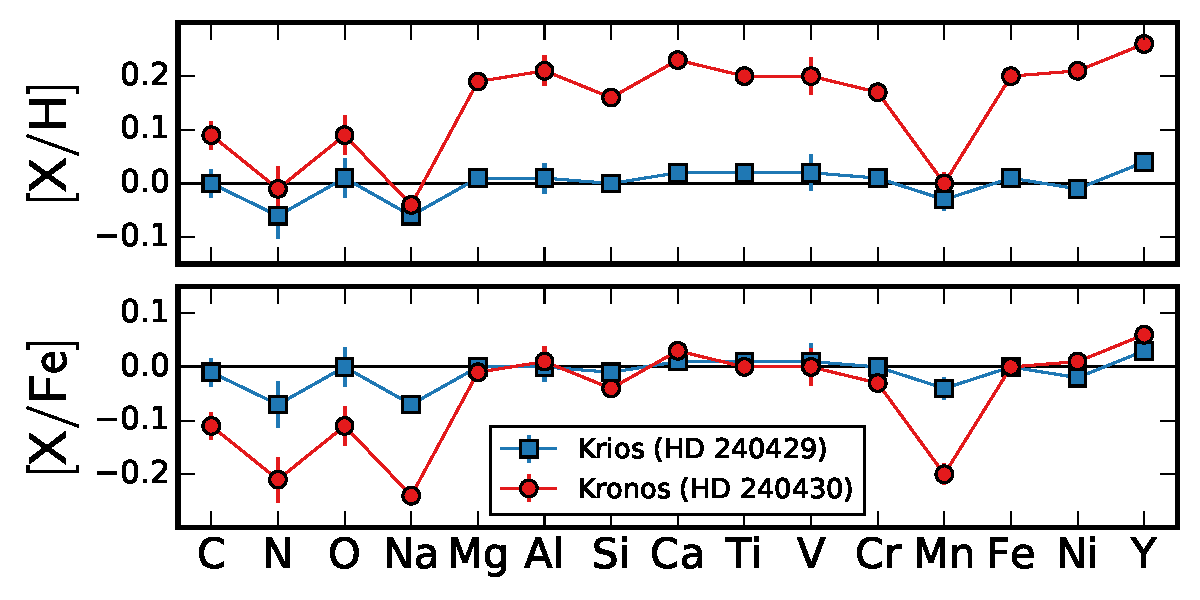
\includegraphics[width=0.9\linewidth]{abundances.pdf}
  \caption{Abundances of the comoving pair, \sunanalog\ and \bizarreone,
    normalized to \elem{H} (top) and \elem{Fe} (bottom).
    Lines are drawn for each star only to guide the eye.
    \bizarreone\ is enhanced in \elem{Fe} by $\approx 0.2$~dex relative to
    \sunanalog\ along with \elem{Mg}, \elem{Al}, \elem{Si}, \elem{Ca},
    \elem{Ti}, \elem{V}, \elem{Cr}, \elem{Ni}, \elem{Y} yet not in \elem{C},
    \elem{N}, \elem{O}, \elem{Na}, and \elem{Mn}.
  }
  \label{fig:abundances}
\end{figure}

\begin{figure}[htpb]
  \centering
  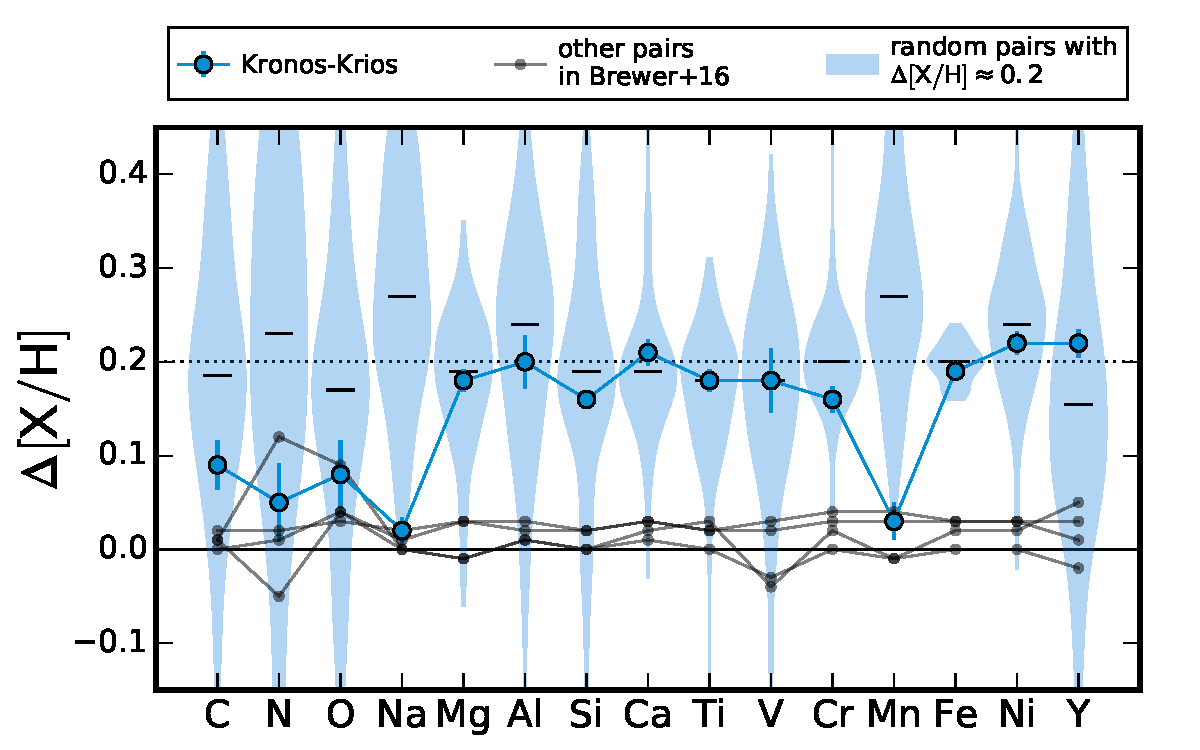
\includegraphics[width=0.95\linewidth]{deltaXH_elem_violins.pdf}
  \caption{Abundance difference in this pair and other twin-like
    ($\Delta T_\mathrm{eff}\lesssim 100$~K) wide binaries in
    \citealt{2016ApJS..225...32B}.
    The differences in other pairs are small ($<0.05$~dex)
    for all elements except \elem{N} and \elem{O} which are the most
    uncertain, making the difference of $\approx 0.2$~dex seen in
    \bizarreone-\sunanalog\ rare.
    Additionally, we show the distribution of abundance differences
    between field stars with similar metallicity difference
    ($\Delta[\elem{Fe}/\elem{H}] \approx 0.2$)
    as violins with medians indicated by black line segments.
    These are random pairings of single stars in
    in \citealt{2016ApJS..225...32B} at two metallicity bins,
    $-0.025 < \feh < 0.025$ (160 stars) and $1.975 > \feh > 2.025$ (137 stars),
    similar to \bizarreone\ and \sunanalog.
    The difference is always taken to be
    $\mathrm{higher}\,\feh - \mathrm{lower}\,\feh$.
    Thus, the narrower range of in $\Delta\feh$ is by construction.
    Random pairings of disk stars with similar $\Delta\feh$ usually show
    similar enhancement in all other elements
    unlike the pattern seen in \bizarreone-\sunanalog\ pair.
  }
  \label{fig:deltaXH}
\end{figure}

\begin{figure}[htpb]
  \centering
  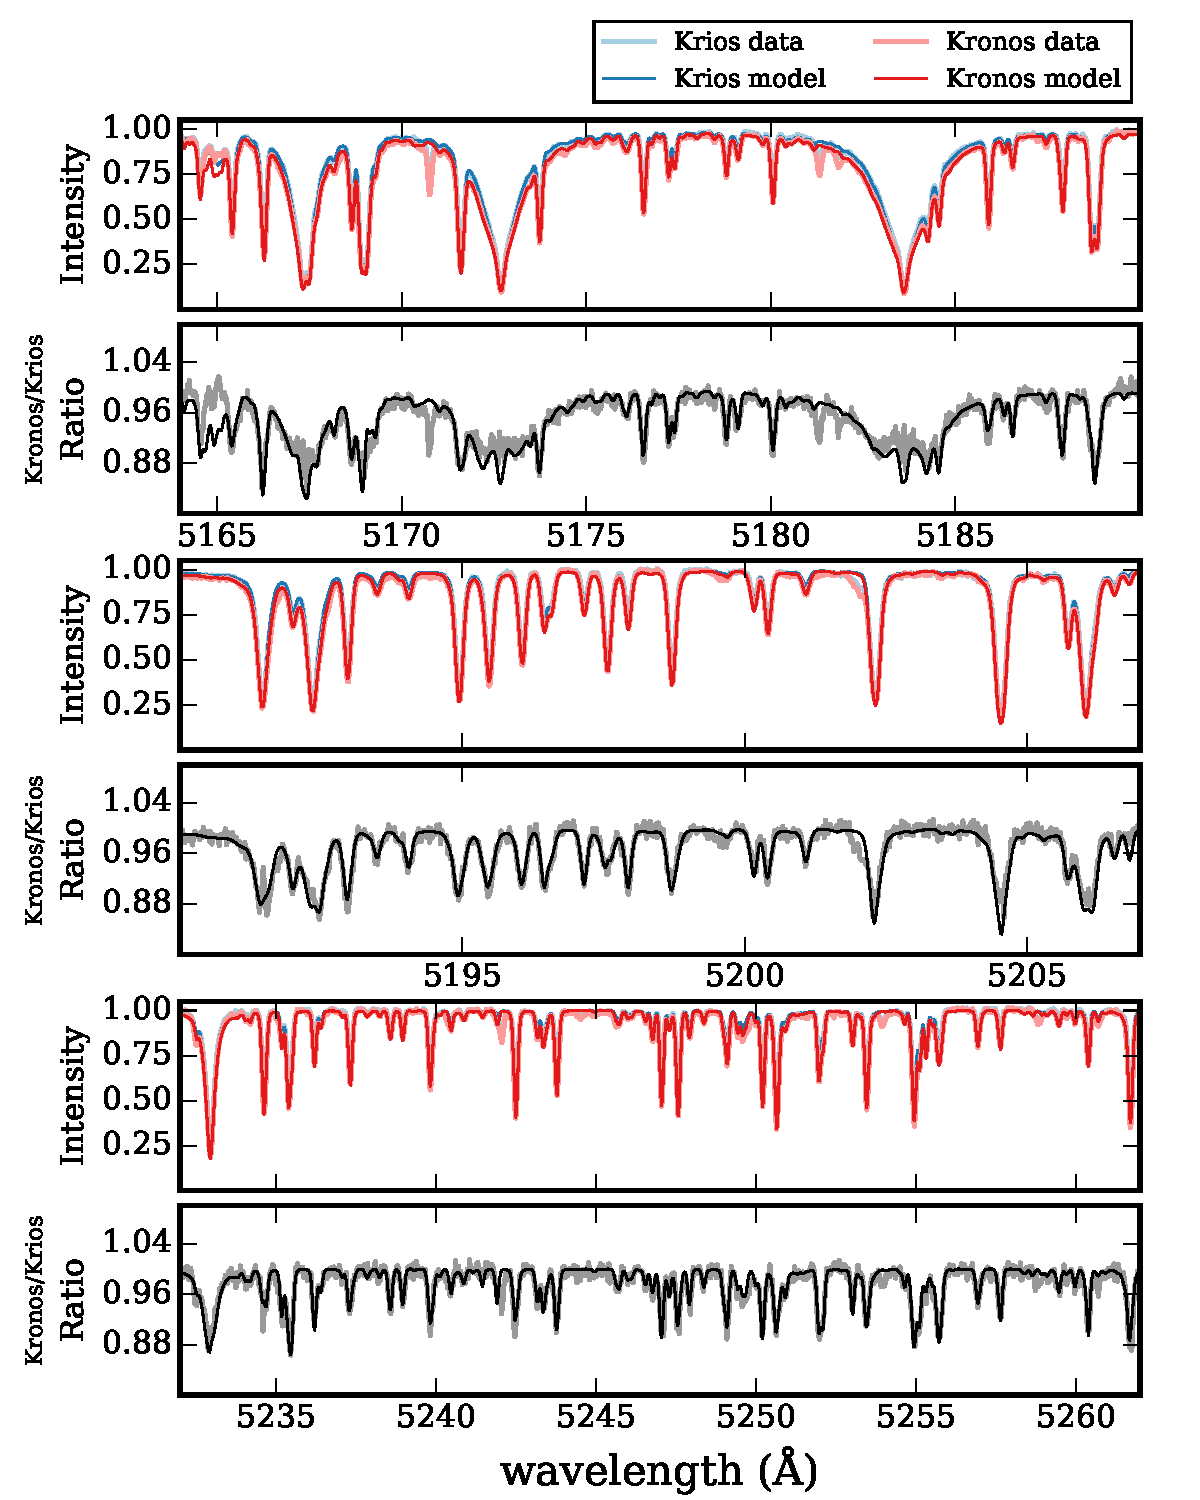
\includegraphics[width=0.95\linewidth]{spec1.pdf}
  \caption{Selective segments of the spectra of \sunanalog\ and \bizarreone.
    Alternating sets of two rows show
    the continuum-normalized data and model in the upper panel,
    and the ratio (\bizarreone/\sunanalog) of data (gray) and model (black)
    in the lower panel.
  }
  \label{fig:spec1}
\end{figure}

\begin{figure}[htpb]
  \centering
  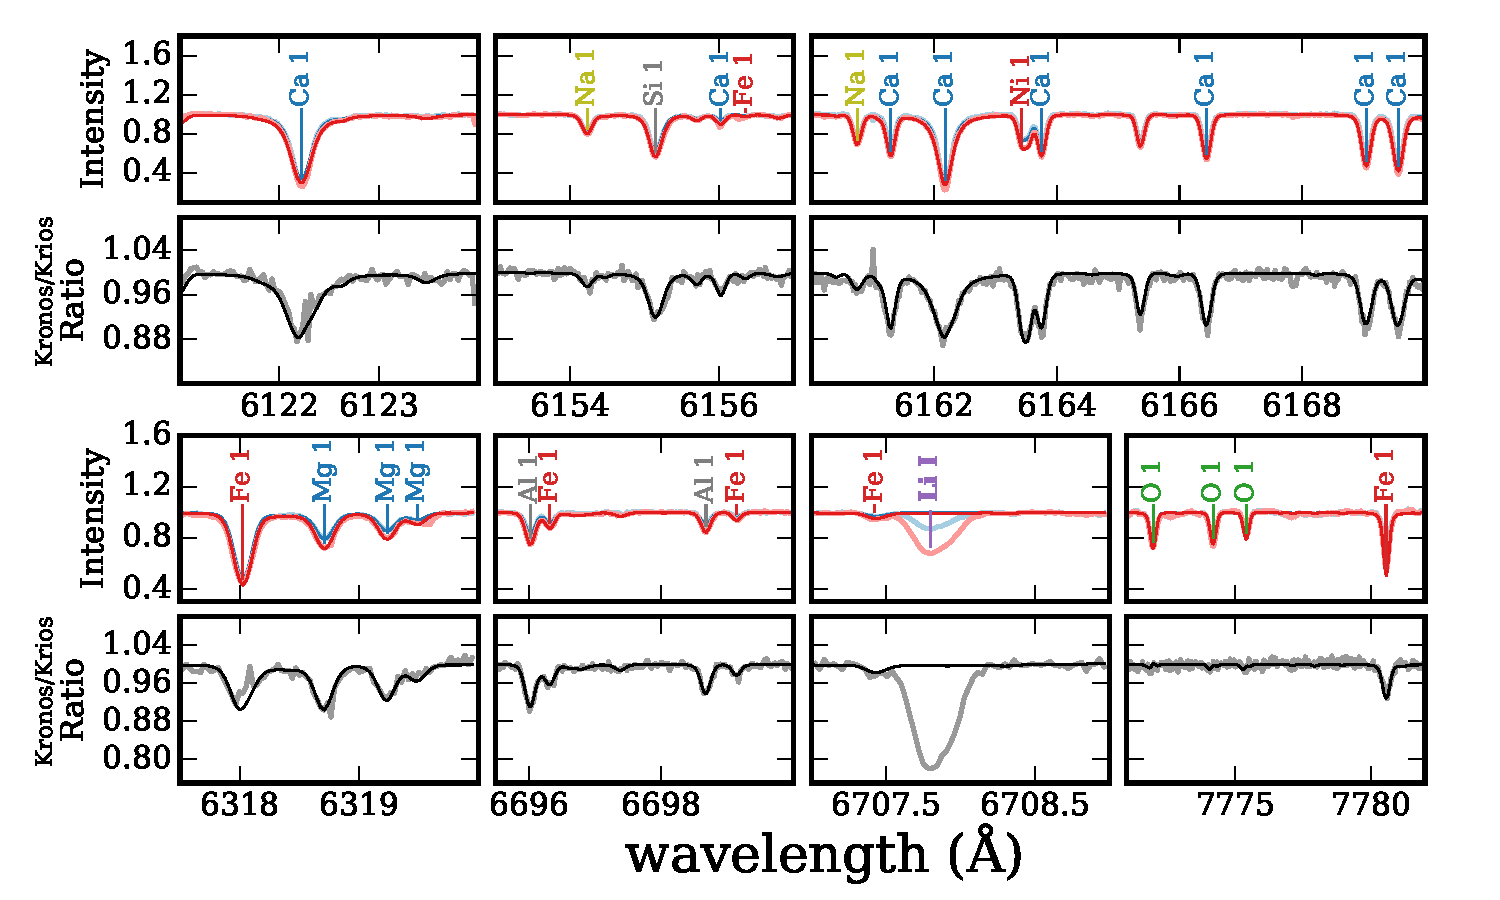
\includegraphics[width=0.95\linewidth]{spec2.pdf}
  \caption{Same as \figname~\ref{fig:spec1}
    but for smaller portions of spectra at longer wavelengths that are
    not dominated by \elem{Fe}.
    We mark elements that give rise to strong absorption lines.
    The feature in the third column of the second row is a strong \elem{Li}
    line that was not modeled by \citealt{2016ApJS..225...32B}; this line was
    studied in a separate work (\citealt{jmlithium}).
    Note that the lines of \elem{Na} and \elem{O}, which are under-enhanced
    in \bizarreone\ relative to \elem{Fe} or other refractory elements,
    show weaker residuals.
  }
  \label{fig:spec2}
\end{figure}

\sunanalog\ and \bizarreone\ were identified as a
candidate comoving star pair in our recent search for comoving stars using the
proper motions and parallaxes from the \tgas\ catalog, a component of \gaia\ \dr\
(the astrometric measurements are listed in \tablename~\ref{tab:kk}).
We refer the readers to this previous work (\citealt{2017AJ....153..257O}) for a
full explanation of the methodology behind this search and only briefly describe
the method here.
For a given pair, we compute a marginalized likelihood ratio between the
hypotheses (1) that a given pair of stars share the same 3D velocity vector, and
(2) that they have independent 3D velocity vectors, both given only observations
of two components of the velocities (parallaxes and proper motions).
We then select a sample of high-confidence comoving star pairs by making a
conservative cut on this likelihood ratio.
In the resulting catalog of comoving pairs (\citealt{2017AJ....153..257O}),
the pair presented in this paper was assigned a group id of 1199,
and the marginalized likelihood ratio (Bayes factor)
between the two hypotheses is $\ln{\mathcal{L}_1/\mathcal{L}_2} = 8.52$,
well above the adopted cut value of 6.
The pair has also been previously recognized as a visual double star system
in Washington Double Star catalog (\citealt{2001AJ....122.3466M}).
We have checked that we do not find any possible additional comoving companions
by lowering the likelihood ratio cut for the stars around this pair.

In a separate effort to study detailed chemical abundances of potential
planet-hosting stars, \citet{2016ApJS..225...32B} obtained and analyzed high resolution
spectra of both stars using the HIRES spectrograph on the Keck~I telescope.
The spectral resolution is $R\approx 70000$ and the wavelength coverage is
$5164--7799$~\AA.
A typical signal-to-noise ratio in the spectral continuum is $>200$~per pixel.
The resulting measurements include elemental abundances for 15 chemical species
(C, N, O, Na, Mg, Al, Si, Ca, Ti, V, Cr, Mn, Fe, Ni, Y) as well as stellar parameters
and high precision radial velocities.
For the details of the spectral analysis, we refer the readers to
\citealt{2016ApJS..225...32B}.
The \elem{Li} doublet at $6707.6$~\AA\ --- clearly visible in both spectra (see
\figname~\ref{fig:spec2}) --- for this sample was investigated in a separate
work (\citealt{jmlithium}).
We list all spectroscopic measurements including
the absolute abundance\footnote{
  The absolute abundance of element \elem{X} is
  $A(\elem{X}) = \log_{10} (n_\elem{X}/n_\elem{H})$
  where $n_\elem{X}$ is the number density of element \elem{X}.
}
of \elem{Li} for the two stars in Table~\ref{tab:kk}.

The projected separation between the pair is 1.9\arcmin\ ($\approx 0.01$~pc),
and the 3D separation is $\approx 0.6$~pc.
Although selected based only on their astrometry, the two stars
have identical radial velocities within uncertainties (Table~\ref{tab:kk}),
confirming that they are truly comoving.
Combining these precise radial velocities with the \gaia\ \tgas\ astrometry, we
can compare differences between the inferred 6D phase space coordinates of the
two stars.
We start by generating posterior samples over the Heliocentric distance, $r$,
tangential velocities, $(v_\alpha, v_\delta)$, and radial velocity, $\hat{v}_r$,
given the observed parallax, $\pi$, and proper motion components,
$(\mu_{\alpha^*}, \mu_\delta)$, and radial velocity, $v_r$.
By defining the vectors
% SMOH: I understand you meant hat v_r as the latent true radial velocity but
% personally think a) it can confuse some people that there are hat quantities
% with no-hat quantities for hat-y vector and thus b) it'd be better to use hat
% quantities for observed variables and no-hat for latent true ones.
% SMOH: v_r is missing in the LHS of eq(3)
\begin{eqnarray}
  \vec{y} &=&
      \transp{\left(
        \begin{array}{c@{\hspace{1em}} c@{\hspace{1em}} c@{\hspace{1em}} c}
          \pi &
          \mu_{\alpha^*} &
          \mu_\delta &
          v_r
        \end{array}
      \right)}\\
  \hat{\vec{y}} &=&
      \transp{\left(
        \begin{array}{c@{\hspace{1em}} c@{\hspace{1em}} c@{\hspace{1em}} c}
          r^{-1} &
          r^{-1}\,v_\alpha &
          r^{-1}\,v_\delta &
          \hat{v}_r
        \end{array}
      \right)}
\end{eqnarray}
and by considering the covariance matrix $\mat{C}$ between the observed
quantities (provided by \tgas\ and extended to include the uncorrelated radial
velocity uncertainty), the likelihood can be written
\begin{eqnarray}
p(\pi, \mu_{\alpha^*}, \mu_\delta \given r, v_\alpha, v_\delta) &=&
  \left[\det\left(\frac{\mat{C}^{-1}}{2\pi}\right)\right]^{1/2} \,
    \exp \left[ -\frac{1}{2} \transp{\left(\vec{y} - \hat{\vec{y}} \right)} \,
    \mat{C}^{-1} \,
    \left(\vec{y} - \hat{\vec{y}} \right) \right] \label{eq:likefn} \quad .
\end{eqnarray}
We adopt a uniform space density prior for the distance and an isotropic
Gaussian for any velocity component, $v$, with a dispersion $\sigma_v=25~\kms$
\begin{eqnarray}
p(r) &=&
  \begin{cases}
    \frac{3}{r_{\rm lim}^3} \, r^2 & \text{if } 0 < r < r_{\rm lim}\\
    0              & \text{otherwise}
  \end{cases}\\
p(v) &=& \frac{1}{\sqrt{2\pi}\,\sigma_v} \,
  \exp\left[-\frac{1}{2} \, \frac{v^2}{\sigma_v^2} \right] \quad .
\end{eqnarray}
For each of the two stars, we use \project{emcee}
(\citealt{Foreman-Mackey:2013}) to generate posterior samples in $(r, v_\alpha,
v_\delta, \hat{v}_r)$ by running 64 walkers for 4608 steps and discarding the
first 512 steps as the burn-in period.
For each sample, we convert the heliocentric phase-space coordinates into
Galactocentric coordinates assuming the Sun's position and velocity are $x_\odot
= (-8.3, 0, 0)~{\rm kpc}$ and $v_\odot = (10, 244, 7.17)~\kms$ (\citealt{bovy,
etc.}).
\figurename~\ref{fig:dxdv} shows differences in posterior samples converted to
Galactocentric phase-space coordinates for the two stars.
In all components, the pair is consistent with being co-moving and close in
separation; the sky-projected separation of the two stars is $\approx$$0.01~\pc$
but the median 3-space separation is $\approx$$0.6~\pc$.

\begin{figure}[htbp]
  \begin{center}
    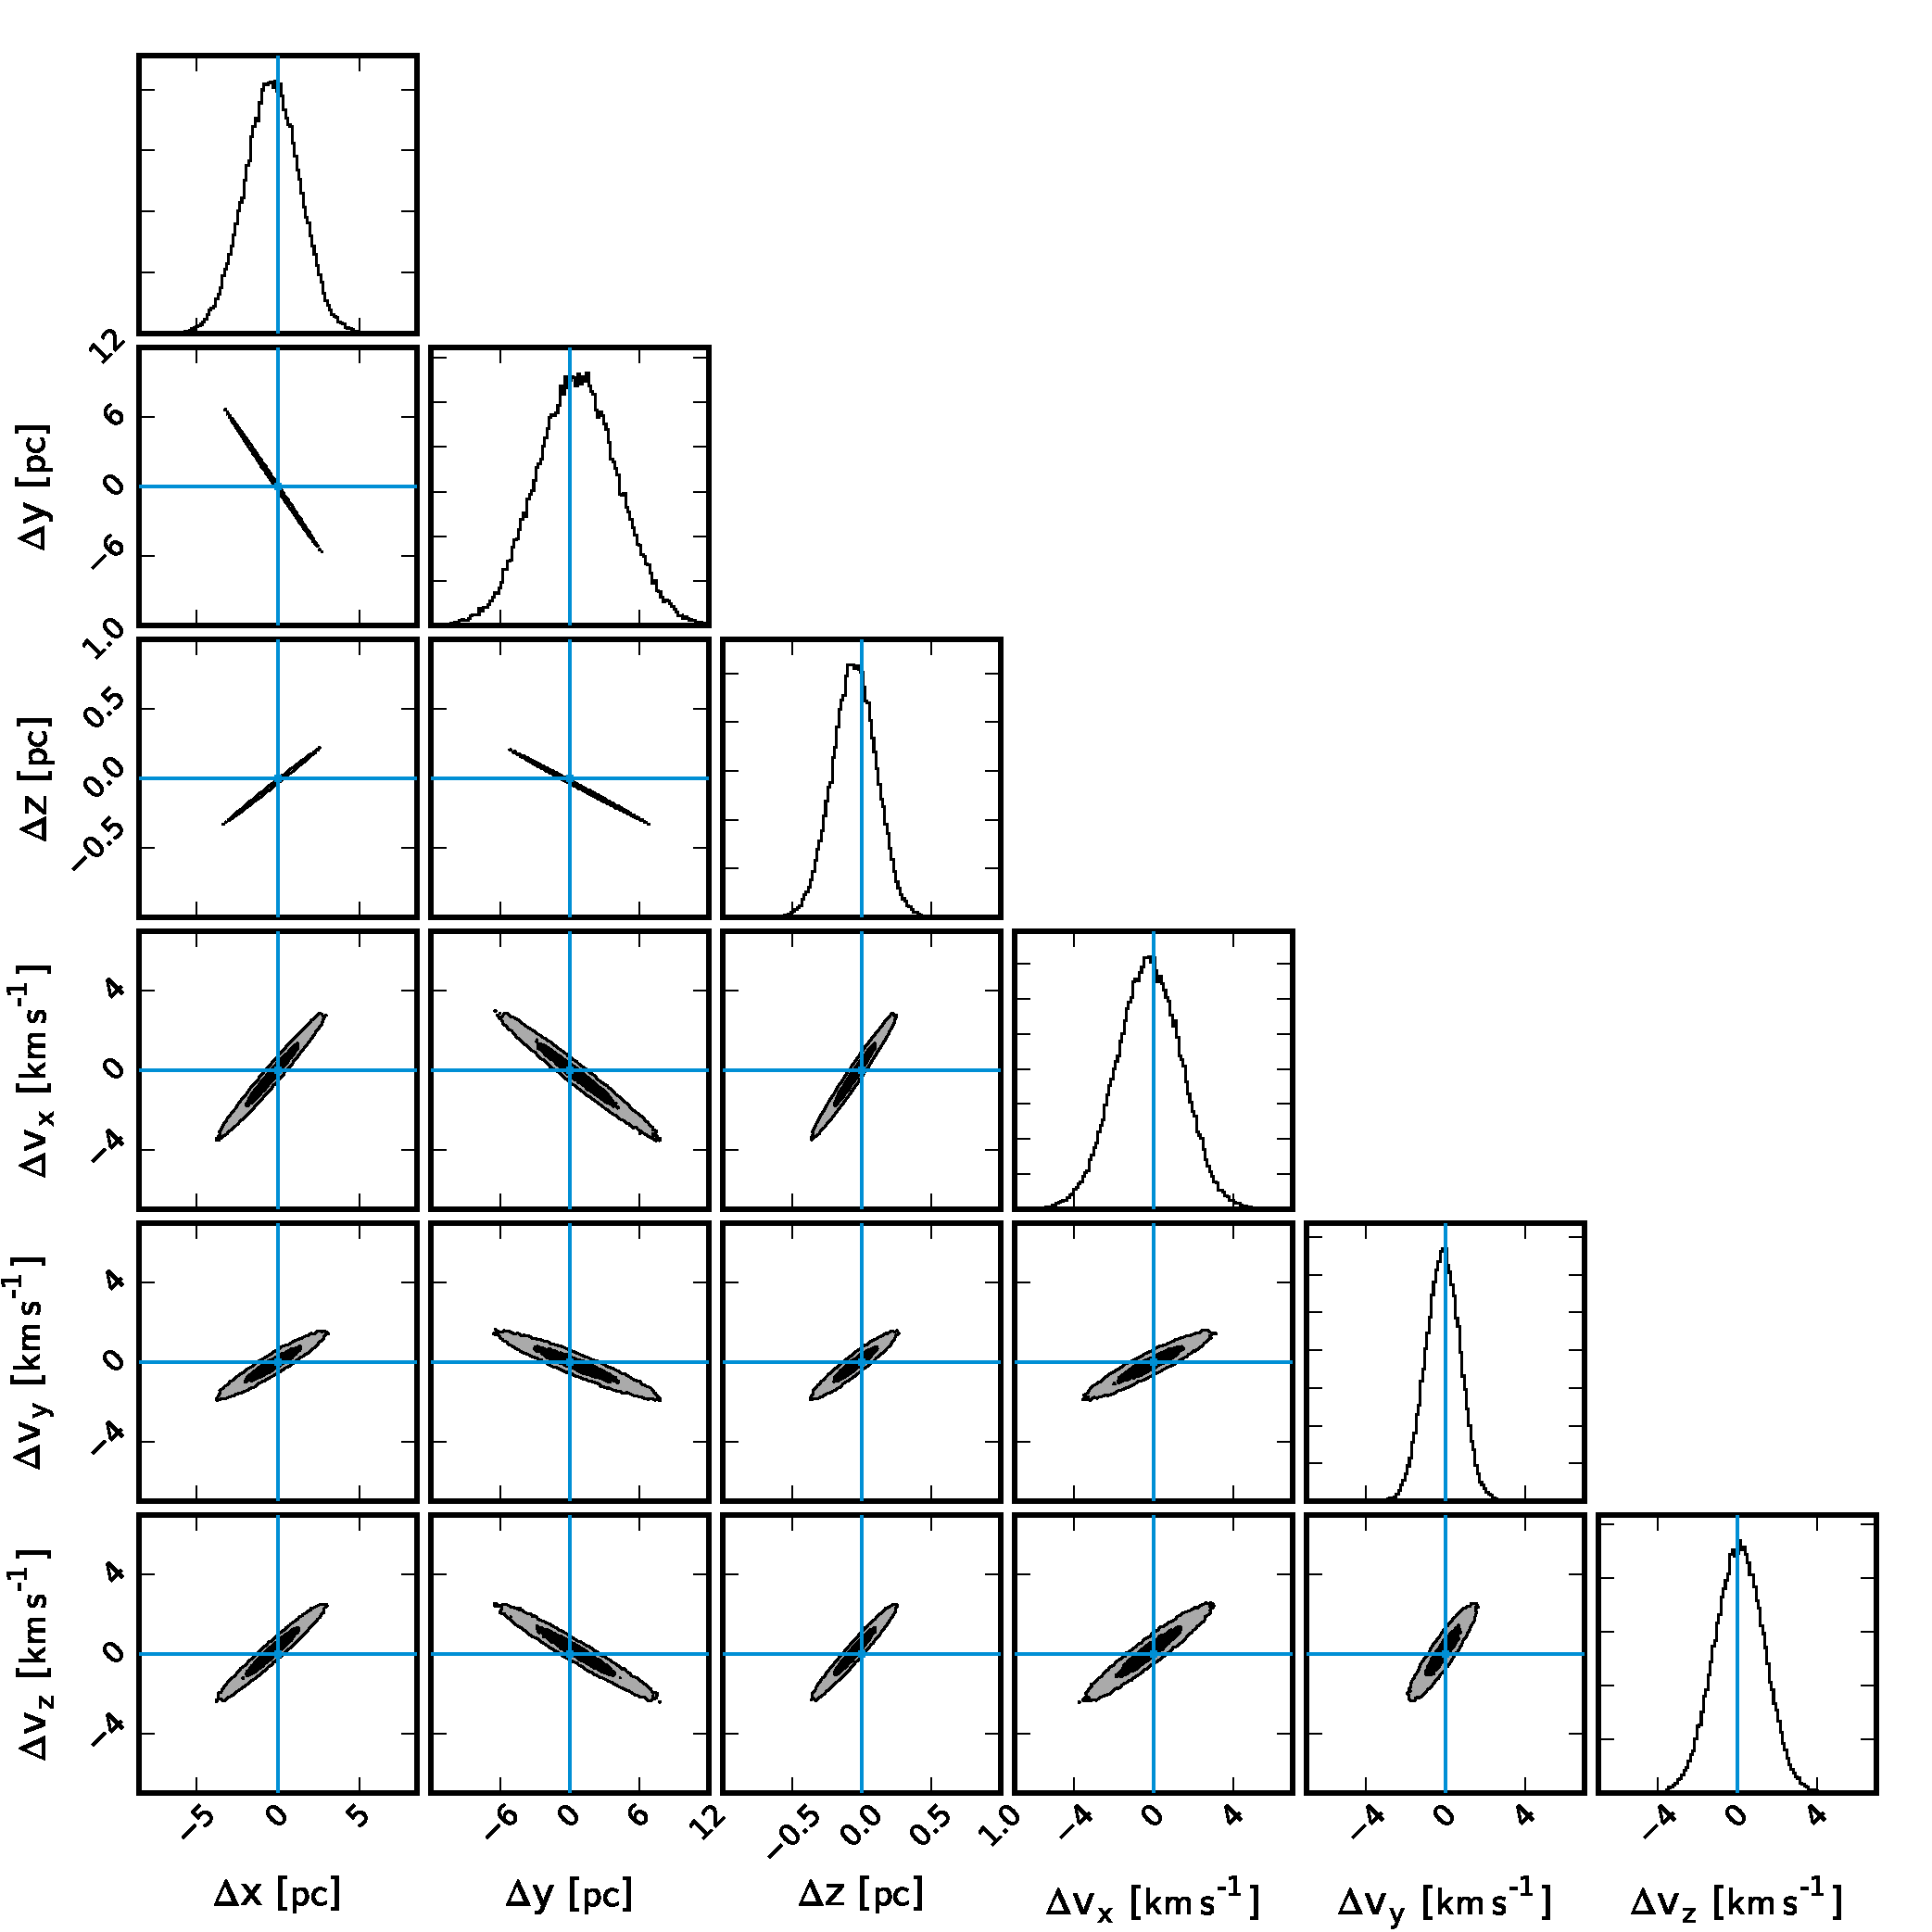
\includegraphics[width=\linewidth]{dx_dv_posterior.pdf}
  \end{center}
  \caption{%
    Differences in posterior samples over Galactocentric phase-space coordinates
    for the two stars \sunanalog\ and \bizarreone.
    \label{fig:dxdv}}
\end{figure}

Given their proximity in phase space, it is generally accepted to assume that
the two stars were born together and, perhaps, are a bound wide binary system.
Thus, we expect the two stars to have identical metallicities and abundance patterns.
Surprisingly, one of the stars, \bizarreone\ is significantly more metal
rich than the other (by 0.2~dex $\approx 60\%$; \figname~\ref{fig:abundances}).
Even more puzzling is that not all elements are equally enhanced:
the abundances of \bizarreone\ show selective depletion in
\elem{C}, \elem{N}, \elem{O}, \elem{Na}, and \elem{Mn}
relative to \elem{Fe}.

The validity of the measured abundance differences is further demonstrated
in \figname~\ref{fig:spec1} and \ref{fig:spec2} where we show
segments of the spectra and models of the two stars
used to measure their abundances.
As expected from their reported metallicity difference ($\Delta\feh \approx 0.2$),
the ratio of data and model between the two stars show significant
residuals of almost all metal line features, largely dominated by \elem{Fe}.
However, for lines of elements that are not as enhanced in \bizarreone\,
the residuals are much smaller in amplitude.
%Li?


We stress that none of the other four twin-like ($\Delta T_\mathrm{eff}
\lesssim 100$~K) wide binary pairs examined in \citealt{2016ApJS..225...32B}
show discrepancies in abundances between the stars at this level.
As shown in \figname~\ref{fig:deltaXH},
the differences in other pairs for all elements except \elem{N} and \elem{O},
which are also the most uncertain (\tablename~\ref{tab:kk}),
are less than $0.05$~dex, making \bizarreone-\sunanalog\ pair a significant outlier.

The abundance differences cannot be due to different chemical enrichment
histories in the disk even if the two stars were of different origin.
\figname~\ref{fig:deltaXH} additionally shows the distribution of abundance
differences, $\Delta[\elem{X}/\elem{H}]$, between random pairings of two stars
with similar \feh\ as \bizarreone\ and \sunanalog\.
We see that when a star is enhanced in $\elem{Fe}$ by $0.2$~dex,
all other elements are typically enhanced at a similar level, with some variations.
Specifically, for a typical star with $\feh \approx 0.2$~dex,
we generally expect $[\elem{Na}/\elem{Fe}] > 0$ and $[\elem{Mn}/\elem{Fe}] > -0.1$
(\citealt{Battistini:2015aa,Bensby:2003aa})
making the low [\elem{Na}/\elem{Fe}] and [\elem{Mn}/\elem{Fe}] seen in \bizarreone\
very unlikely to arise from variations in Galactic chemical evolution.

% HOGG to provide some theoretical account adding to the above empirical evidence.



\begin{figure}[htpb]
  \centering
  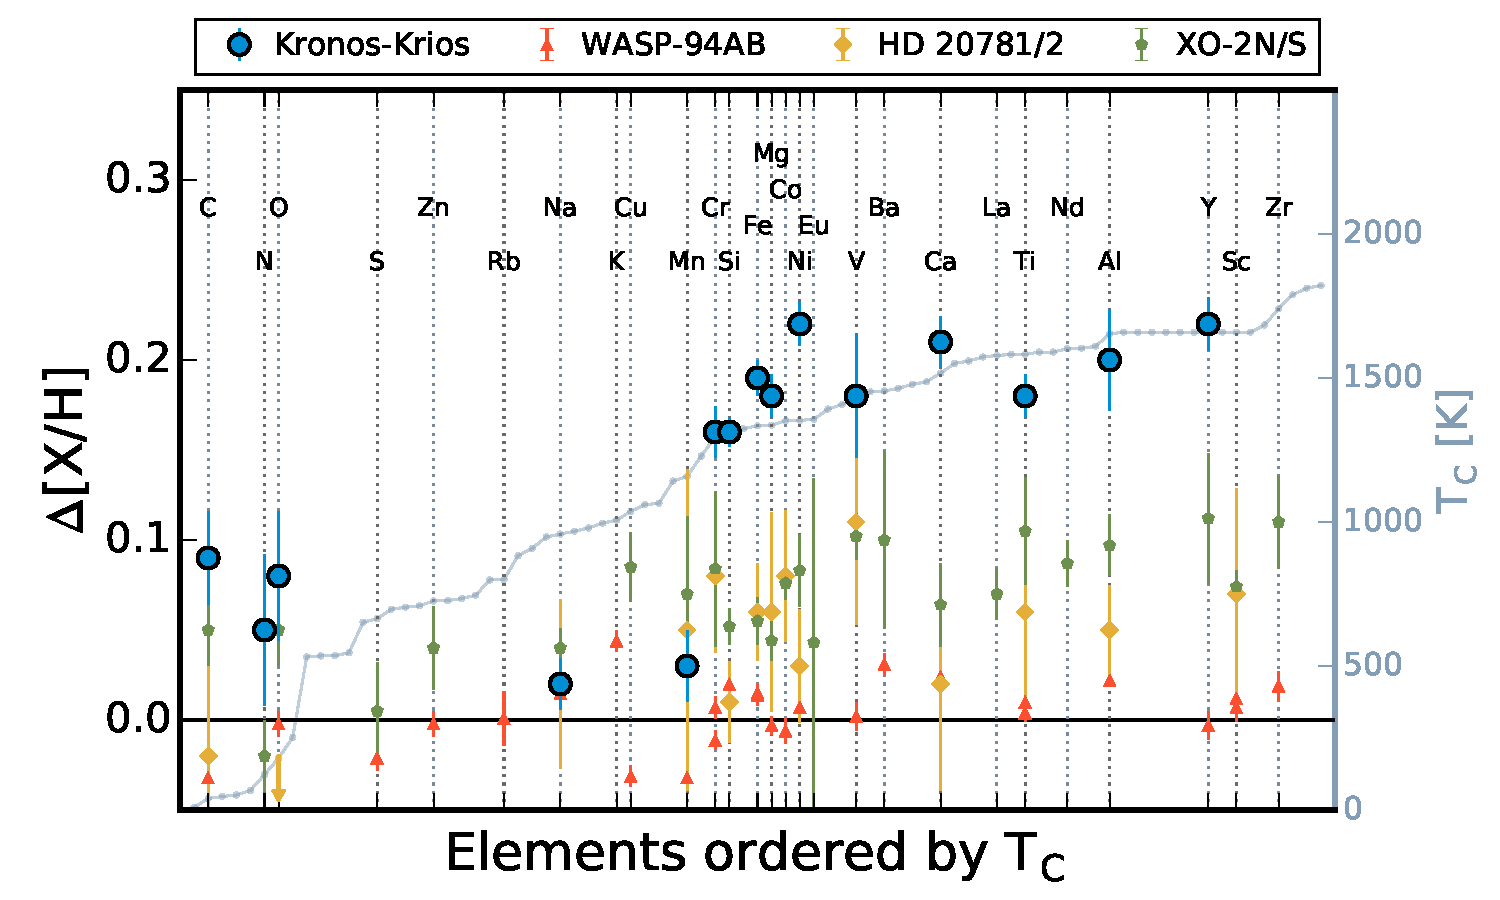
\includegraphics[width=0.95\linewidth]{TcRank_deltaXH_concise.pdf}
  \caption{Abundance differences of the \bizarreone-\sunanalog\ pair
    ranked by the condensation temperature of elements for solar composition gas
    from \citealt{2003ApJ...591.1220L}.
    The condensation temperature may be read from the gray line and right y-axis.
    We show three wide binary systems selected from the literature:
    HD~20782/1 (\citealt{Mack:2014aa}, $\feh\approx0$),
    XO-2N/S (\citealt{Biazzo:2015aa}, $\feh\approx0.35$),
    and WASP-94AB (\citealt{Teske:2016aa}, $\feh\approx0.3$).
    Locations of elements with at least one measurement from any study
    are indicated by a vertical line and its symbol.
    Note that often multiple values are reported for one element corresponding
    to different ionization states in equivalent width analyses.
    No other pair studied so far were shown to have such large difference
    in metallicity or sharp contrast between (moderately) volatile and
    refractory elements as \bizarreone-\sunanalog.
  }
  \label{fig:relabun_tcrank}
\end{figure}


\section{Discussion}
\label{sec:discussion}

We discuss the possible origins of the peculiar abundance differences of
\bizarreone-\sunanalog.
Although the data described above strongly suggests that the two stars are
coeval, let us first consider scenarios in which the two stars are not actually
born together.

% chance pair
%Given that their metallicities and abundance patterns are significantly
%different, one may simply conclude that the two stars are not related (coeval)
%but they merely happen to be comoving at such small separation ($\approx 0.6$~pc)
%by chance.
%The two stars are in the Galactic disk, and assuming certain velocity ellipsoid
%at the stars' location, one may compute the probability that a star moving at
%the mean velocity of the two stars would have a companion within $\Delta v = XX$~km/s.
%...

\subsection{Stellar Ages \& Coevality}
\label{sub:ages}

The fact that the two stars share a nearly identical space motion
at a separation of $< 1$~pc strongly argues that the pair is coeval.
We therefore  consider other age indicators apart from their phase space coordinates
to assess the ages and coevality of the two stars.
First, given the precise measurements of $\log(g)$ and $T_\mathrm{eff}$,
we can constrain the ages of the two stars by
comparing these values to theoretical isochrones.
We perform isochrone fitting to these values using the Yale-Yonsei model
isochrones (\citealt{2013ApJ...776...87S}).
The input data are $\log(g)$, $T_\mathrm{eff}$, \feh,
parallaxes, $B$-band magnitudes, and their errors.
The best-fit isochrone ages of \sunanalog\ and \bizarreone\ are
$4.00_{-1.56}^{+1.51}$~Gyr and $4.28_{-1.03}^{+1.11}$~Gyr, respectively,
consistent with them being coeval.

The surface lithium abundance in a sun-like star decreases with its age due to
mixing induced by convection or rotation, which brings the lithium into the
interior ($T>2.5 \times 10^{6}$~K) where it will be destroyed by proton capture
burning.
Thus, surface lithium abundance is an indicator of stellar ages.
The absolute $\elem{Li}$ abundance of $2.25$~dex for \sunanalog\ implies an age
of $\lesssim 1$~Gyr according to the theoretical models tuned to explain the
solar lithium abundance and rotational profile (\citealt{2005Sci...309.2189C}).
The lithium abundance of \bizarreone\, $2.74$~dex, shows the largest difference
among all measured elements.
This translates to a $\sim 500$~Myr difference in age.
Given the overall higher metal abundances and the peculiar abundance patterns
in \bizarreone, it is unclear, however, whether this higher $\elem{Li}$
abundance means a younger age or something else.
For example, the presence of $\elem{Li}$-rich red giant stars has been
attributed to the engulfment of substellar companions such as gas giant planets
or brown dwarfs which may replenish $\elem{Li}$ (\citealt{Casey:2016aa}).

In fact, the surface lithium abundance is the only indication that points to younger ages.
If the two stars are indeed only several hundred Myrs old at most,
they are expected to be part of a larger comoving group of stars.
However, as we mention above, there is no evidence in our search of comoving pairs
using \tgas\ that the two stars belong to a larger group of young stars.
Very young stars are often show signs of activity such as
X-ray emission from magnetic activity, emission lines, or infrared excess due to
circumstellar disks.
We have looked for these signs for the pair to find none, and their spectral energy
distributions are consistent with blackbody.
The low $v\sin(i)$ values (\tablename~\ref{tab:kk}) also argue against very
young ages inferred from the surface lithium abundances.
% TODO: reference for vertical action as age?
Finally, the pair's fiducial orbit in a axisymmetric Milky Way-like potential
has a vertical action larger than the Sun, favoring an older age.
We therefore conclude that the two stars are most likely coeval, $\sim 4$~Gyr old main
sequence stars, and that their unusually high \elem{Li} abundance requires an
alternative explanation.

\figurename~\ref{fig:orbit} shows an orbit computed from the median posterior
sample over 6D phase-space coordinates for \sunanalog\ (black line), integrated
in a Milky Way-like gravitational potential (\cite{Gala:2017}). \todo{APW:
explain}
The Sun's orbit in this same Milky Way model is under-plotted for comparison
(grey line); the orbits of the stars in this pair have large scale-heights
relative to the Sun's orbit despite being young.

\begin{figure}[htbp]
  \begin{center}
    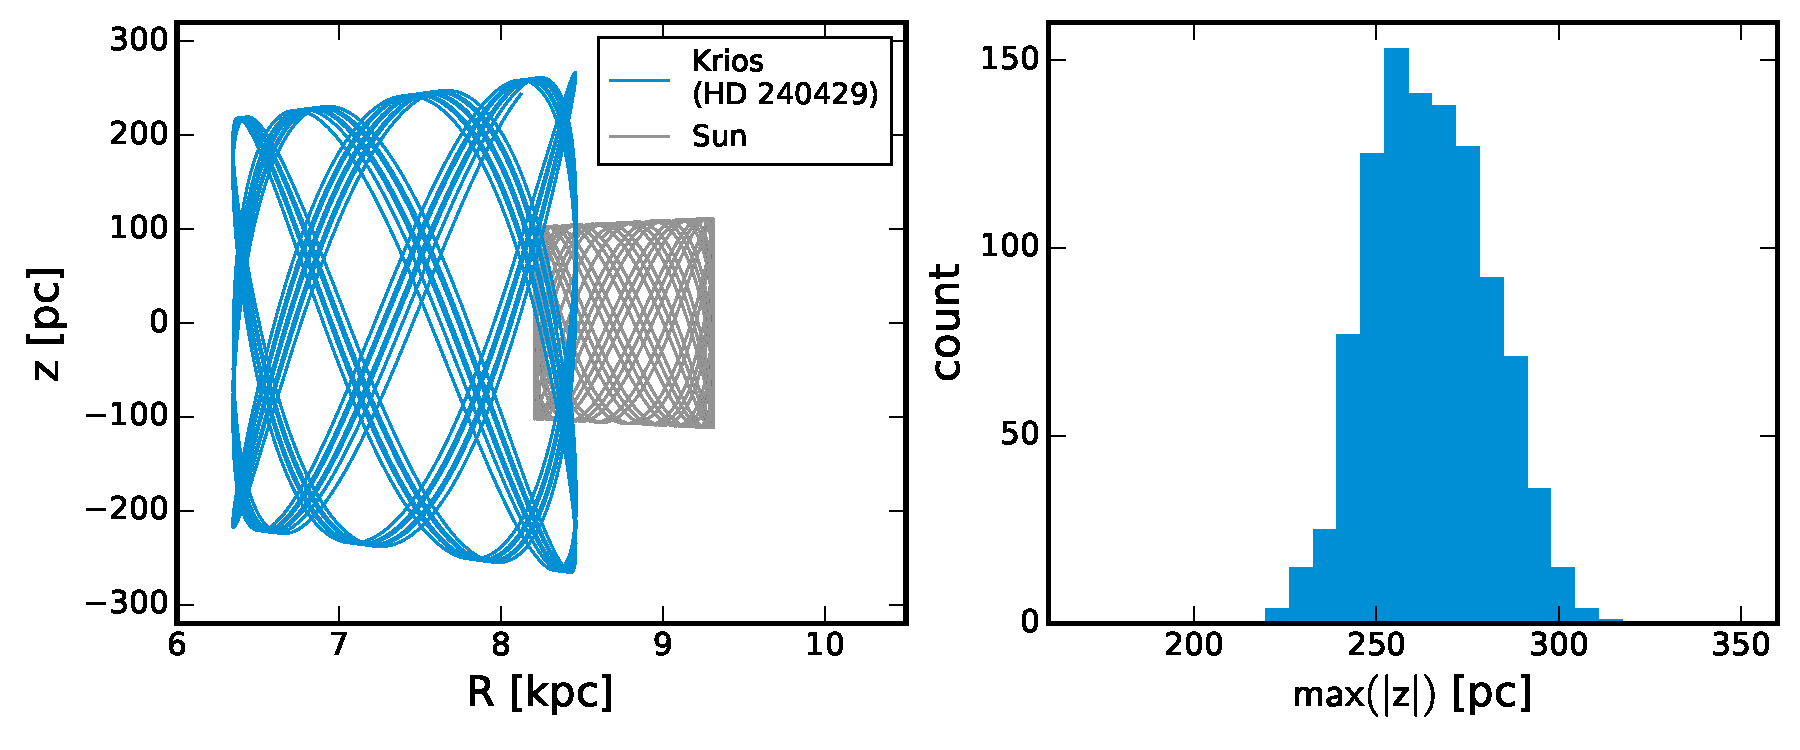
\includegraphics[width=\linewidth]{orbits.pdf}
  \end{center}
  \caption{%
    Galactic orbits computed for \sunanalog\ (black) and the Sun (grey).
    For \sunanalog\, the initial conditions are set to the median posterior
    sample over the inferred 6D phase-space coordinates.
    The orbits are computed by integrating backwards from the present-day
    positions for $2.5~{\rm Gyr}$ with a time-step of $0.5~{\rm Myr}$ using the
    Leapfrog integration scheme implemented in \project{Gala}
    (\citealt{Gala:2017}). \todo{APW: citation...}
\label{fig:orbit}}
\end{figure}


\subsection{Exchange Scattering}
\label{sub:exchange_scattering}

% binary-single and binary-binary exchange
Two stars unrelated at birth may end up in a binary system via binary-single scattering event
that results in an exchange of binary member.
In order to estimate the rate at which any binary-single
event will produce a wide binary system such as \sunanalog\ and \bizarreone,
we may consider the rate at which this wide binary will scatter with a field star to
result in an exchange reaction.
The cross-section of exchange scattering for a binary with semi-major axis $a$ is
\begin{eqnarray}
  \sigma_\mathrm{ex} = \frac{640}{81} \pi a^{2} \frac{1}{v^6}
\end{eqnarray}
where $v$ is the incoming velocity $v_i$ in units of critical velocity $v_c$ defined as
\begin{eqnarray}
  v_c^2 = G \frac{m_1 m_2 (m_1 + m_2 + m_3)}{m_3 (m_1 + m_2)} \frac{1}{a}
\end{eqnarray}
when $v \gg 1$ using the impulse approximation (\citealt{Hut:1983aa,Hut:1983ab}),
which is appropriate for wide binaries scattering with field (disk) stars.
If we assume that field stars are made of solar mass stars
with constant number density $n=1$~pc$^{-3}$, and the incoming velocity of field stars
is $10$~km\,s$^{-1}$, a lower limit to the velocity dispersions of disk
stars in any direction, the rate of exchange scattering is
\begin{eqnarray}
  n \sigma_\mathrm{ex} v_i = 6.82\times 10^{-8}\,\mathrm{Gyr}^{-1}
  \frac{n}{\mathrm{pc}^{-3}} \frac{\mathrm{pc}}{a} \left(\frac{10~\mathrm{km}\,\mathrm{s}^{-1}}{v_i}\right)^5
\end{eqnarray}
low enough to be negligible.
Because the exchange scattering cross section steeply depends on the incoming velocity
relative to the critical velocity (of the order of orbital velocity of the binary),
the rate of exchange scattering with a star within the same star forming region
may be much larger.
However, this, or any other exchange scattering scenario,
is still unsatisfactory as it offers no insight on the
peculiarity of the abundances of \bizarreone\ (see
\sectionname~{\ref{sec:data}}).
In case that the pair formed from an exchange scattering event,
we would expect the pair to be composed of typical field stars,
not one with such low $\elem{Na}/\elem{Fe}$ and $\elem{Mn}/\elem{Fe}$.

%LEIGH to fill in binary-binary exchange scattering?

The unlikeliness of the above possibilities naturally leads us to consider the
alternative that their peculiar disparity in chemical abundance space may be
more naturally explained.


\subsection{Chemical Inhomogeneity in Star Formation}
\label{sub:chemical_inhomogeneity_in_star_formation}

% inhomogeneity in star formation
It may be that the two stars are born at the same time from the same cloud, but
there is chemical inhomogeneity within the cloud.
However, there is already ample amount of evidence against such scenario.
First, none of the other seven similar wide binaries examined in
\citealt{2016ApJS..225...32B} show the same level differences in abundances
although there is generally a larger spread in $\elem{C}$, $\elem{N}$ and
$\elem{O}$, and some pairs show a large as $\approx 0.15$~dex difference in
particular elements.
The median and maximum \feh\ difference between component stars in the other
seven pairs is $0.02$~dex and $0.09$~dex, respectively.
The differences are even smaller (maximum $\Delta\feh = 0.03$~dex)
if we compare only twin-like ($\Delta T_\mathrm{eff} \lesssim 100$~K) pairs.
This is consistent with the findings of \citealt{Desidera:2004aa}, who examined
23 wide binaries of late F to K dwarfs, and found most pairs show difference in
\feh\ less than $0.02$~dex and none larger than $0.07$~dex.
Similarly \citealt{Gratton:2001aa} found that four out of six equal mass binaries
have the same chemical composition with $\gtrsim 0.01$~dex uncertainties.
Thus, a difference of $\approx 0.2$~dex seen in \bizarreone-\sunanalog\ pair
cannot be due to chemical inhomogeneity in the birth cloud.


\subsection{Accretion of rocky planetary material}
\label{sub:accretion}

% rocky planets (or the like) engulfment
Yet another more exotic possibility is that a star's surface abundance may
be altered by accretion of planetary material after birth.
Instabilities may develop in a multi-planet system due to its chaotic nature
which may lead to planet engulfment or ejection by the host star.
%TODO: needs references
%TODO: kozai?
Indeed, it is an important goal of many exoplanet studies
to detect chemical signatures of planet formation or accretion,
distinguish them from Galactic chemical evolution, and
connect them to theories of evolution of planetary systems.
One approach that is free from confusion with Galactic chemical evolution
is to compare two almost identical stars in a wide binary system,
which are assumed to be born together.
Assuming that the component stars were born together with identical
initial composition, we may see a difference in their surface abundances
if the two stars then went through different amount of accretion
of planetary material.
This abundance difference may depend on the condensation temperatures of
elements in the protoplanetary disks from which the accreted planets formed
as their compositions depend on the radial temperature gradient in the disk.
%TODO: cautions on condensation temperature
% 1. it is just a proxy
% 2. it is **equlibrium** condensation temperature

We now turn to \bizarreone-\sunanalog\ pair.
In Figure~\ref{fig:relabun_tcrank}, we show the abundace difference
between \bizarreone\ and \sunanalog\ ordered by the rank of \Tcondens\
of each element.
The equilibrium condensation temperatures for the composition of solar system
are taken from \citealt{2003ApJ...591.1220L} (Table~8).
The difference seen in \bizarreone-\sunanalog\ is
compared to HD~20781/2, XO-2N/S, WASP-94A/B in \figname~\ref{fig:relabun_tcrank}.
The metallicity difference of $\approx 0.2$~dex observed in this pair
is larger than the differences seen in any other pairs studied so far.
%Indeed, some may consider such large difference in metallicity
%enough to concluded that the two stars are completely unrelated.
Strikingly, the five under-enhanced elements in \bizarreone\
relative to \sunanalog\ are the five most volatile in all elements measured.
The difference in \elem{Mn} ($\Tcondens = 1158$~K) and
\elem{Cr} ($\Tcondens = 1296$~K) suggests a break in $\Tcondens \approx 1200$~K.
This $\Tcondens$-dependent trend of $\Delta\elemH{X}$,
combined with the enhanced $\elem{Li}$ abundance ($A(\elem{Li}) = 2.75$),
strongly suggests that accretion of rocky material has occured in \bizarreone.

How much mass of rocky material is needed to explain an increment of $\approx 0.2$~dex?
One can carry out simple toy calculations of expected $\Delta\elemH{X}$
in a Sun-like star's atmosphere when adding material of e.g., bulk Earth composition
under these simplifying assumptions:
\begin{itemize}
  \item The material added is instantly and completely mixed.
  \item The atmospheric composition that we measure is identical throughout
    the star's radiative and convective zone.
  \item The surface abundance of the star has been altered once only by this
    accretion event, and remained the same since.
\end{itemize}

We take the solar abundances $\elemH{X}$ of \citealt{Asplund:2009aa}
which can be converted to mass fraction in each element $X$ as in
\begin{equation}
  f_{X,\mathrm{photo}} = \frac{10^{\elemH{X}} m_X}{\Sigma_X 10^{\elemH{X}} m_X}
\end{equation}
where $m_X$ is the mass of each element in e.g., atomic mass unit.
One can check that the \citealt{Asplund:2009aa} abundances
are consistent with mass fraction in \elem{H}, \elem{He} and metals
$X,\,Y,\,Z=0.757,\,0.249,\,0.0134$ as stated in that work.
Assuming a fraction of the star's convective zone in mass $f_\mathrm{CZ}$,
and that the added material has a total mass $M_\mathrm{add}$ and mass fraction in each
element $f_{X,\mathrm{add}}$,
the abundance difference is
\begin{equation}
  \Delta\elemH{X} = \log_{10} \frac{f_{X,\mathrm{photo}}\,f_\mathrm{CZ}\,M_\mathrm{star} + f_{X,\mathrm{add}}\,M_\mathrm{add}}
    {f_{X,\mathrm{photo}}\,f_\mathrm{CZ}\,M_\mathrm{star}}
\end{equation}
We take the composition of bulk Earth from a chondritic model of the Earth
(\citealt{mcdonough2001composition}).

Figure~\ref{fig:toycalc} shows the expected change of surface abundances of
metals in a Sun-like star after $20~\mearth$ of material with composition of
bulk Earth is added.
It has been long known that compared to CI or other carbonaceous chondrites,
the composition of the Earth shows a volatilaity trend that moderately volatile
elements (including Mn and Na) and volatile elements are incearsingly more
depleted with decreasing condensation temperature
(\citealt{mcdonough2001composition}).
This trend is presumed to be closely related to the formation of terrestrial
planets in particular to the radial temperature gradient in a protoplanetary
disk.
Given the simplistic assumptions laid out above, and the uncertainties in our
current knowledge of the compositions of terrestrial planets including bulk
Earth, the match between our toy calculation and the observed abundance
difference between \bizarreone\ and \sunanalog\ is remarkable.

% some discussion of individual elements

What about \elem{Li}?
The element \elem{Li} is worth a special attention in the context of accretion scenario.
Because Li is present in either carbonaceous chondrites or the bulk Earth with
a concentration of $1-1.5$~ppm in mass (\citealt{mcdonough2001composition}),
but is depleted quickly within the first couple of Gyrs on the surface of a
Sun-like star, accretion of either material at later times will significantly
replenish the lithium on the star's surface.
For the present-day Sun, the accretion of $20~\mearth$ of bulk Earth-like
material results in $\Delta\elemH{Li} \approx 1.6$~dex (which
is indicated as an upward arrow in \figname~\ref{fig:toycalc}).
Incidentally, the star under examination, \bizarreone, has an age (informed by
stellar parameters) very close to the Sun ($4.28_{-1.03}^{+1.11}$~Gyr).
Thus, as long as we believe the Sun's present-day surface \elem{Li} abundance
to be ordinary, this predicts that the \bizarreone\ should have $1.6$~dex enhancement
in its \elem{Li}.
This is in fact exactly what we find: the \elem{Li} abundance of \bizarreone\ is
$A(\elem{Li}) = 2.75$ (Table~\ref{tab:kk}, \citealt{jmlithium})
approximately $1.65$~dex higher than the solar value of $1.1$~dex.
%TODO: solar Li needs reference
Furthermore, this implies that the accretion event should have happened very
recently from a time ago that is shorter than the \elem{Li} depletion time.

%TODO: not sure if this is too obvious of a point or useful in practice..
%It is further worth pointing out that measuring the \elem{Li} abundance
%with some of the refractory elements such as $\elem{Fe}$
%provides a way to estimate the time of the event.
%If the observed \elem{Li} abundance is less than what is inferred from
%abundance differences of other elements, and
%we have a model of \elem{Li} depletion, the time of \elem{Li} enhancement
%may be calculated.

What about \sunanalog?
\sunanalog\ is also enhanced in \elem{Li} considering its age of
$4.00_{-1.56}^{+1.51}$~Gyr than the nominal \elem{Li} depletion predics by
$\approx 1$~dex.
This enhancement puts an upper limit on the accreted mass to be
$\approx 4$~\mearth assuming \elem{Li} concentration of $1.1$~ppm
(\citealt{mcdonough2001composition}).
Unlike \bizarreone, we cannot know the pre-accretion abundances of \sunanalog
\footnote{
  Strictly speaking, we can never know the pre-accretion abundances
  for \bizarreone\ either.
  We only have an {\it approximate} idea that this is not far from a solar-twin
  star \sunanalog, and because the deviation from this ``anchor'' star is
  large, it is reasonable to consider an accretion by the Sun.
  In reality, \sunanalog\ may as well have had its own accretion history,
  which indeed seems to be the case according to its \elem{Li} abundance.
}.
However, we note that the span of abundance difference between highly volatile
elements (\elem{C}, \elem{N}, \elem{O}, \elem{Na}) and refractory elements such
as \elem{Fe} expected from accreting $4$~\mearth to the Sun is $\approx
0.05$~dex.
This is comparable to the abundance difference between N, Na and Fe in
\sunanalog.
It is also interesting that \sunanalog\ also shows a deficit in the same
volatile and moderately volatile elements
(\elem{C}, \elem{N}, \elem{O}, \elem{Na}, and \elem{Mn}) relative to Fe
just as in \bizarreone.
Thus, we conclude that \sunanalog\ is also likely to have had a similar
accretion event, but the amount of accretion was much smaller than \bizarreone.

%TODO: augment this paragraph
% - more geochemical study references
We stress that while the calculation carried out is useful in
order-of-magnitude sense, further investigation of each of the simplifying
assumptions made is warranted.
In addition, the composition of bulk Earth also has some uncertainties.
For example, the reported bulk Earth concentration of the siderphile element
\elem{Mn}, varies from $800$ to $1700$~ppm (\citealt{1998psc..book.....L}).
While the latter value from \citealt{mcdonough2001composition} has been used in
our calculation, the former value would bring the observed $\Delta\elemH{Mn}$
to an even closer agreement.
Given these limitations, the level of agreement for the refractory {\it and}
\elem{Li} for \bizarreone\ is remarkable.

\begin{figure}[htpb]
  \centering
  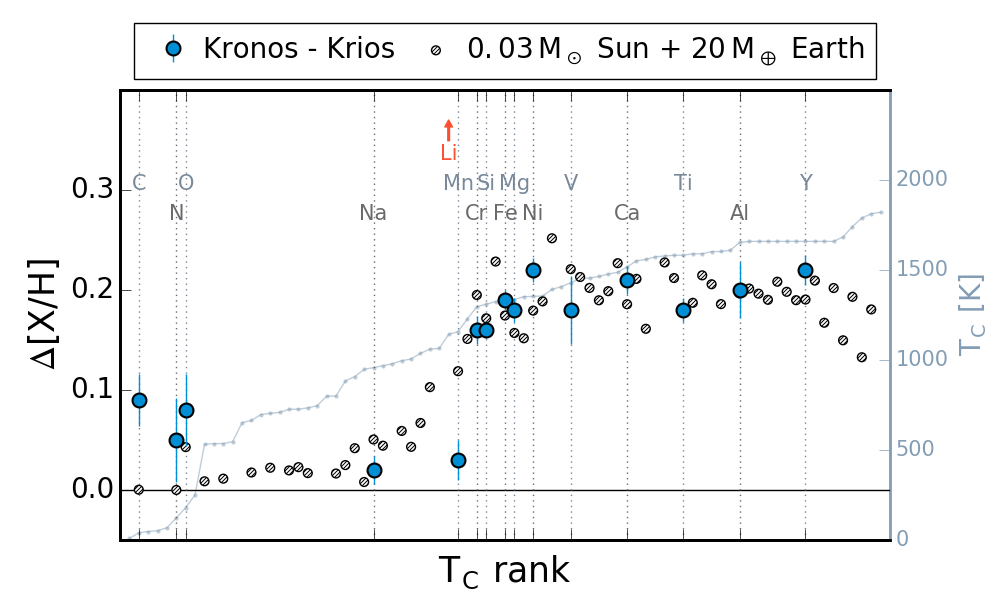
\includegraphics[width=0.95\linewidth]{toycalc.png}
  \caption{
    Comparing the observed abundance difference vs. \Tcondens\ rank
    to the expected change in solar surface abundance after adding $20$~\mearth\ of
    material with bulk Earth composition (\citealt{mcdonough2001composition}).
    The assumed mass fraction in the convective zone is $0.03$.
    All metals are ranked by their \Tcondens\ for solar composition gas,
    and the condensation temperature may be read from the gray line and right y-axis,
    same as in \figname~\ref{fig:relabun_tcrank}.
    Locations of the elements measured for \bizarreone-\sunanalog\ pair are
    indicated by a vertical line and its symbol.
    The close match with the observed abundance difference in \bizarreone-\sunanalog\ pair
    suggests that the abundance difference may be due to accretion of
    $20$~\mearth\ of rocky planetary material.
    The element \elem{Li} is off the plot and indicated with a red arrow
    (see text for details).
  }
  \label{fig:toycalc}
\end{figure}


\section{Summary}
\label{sec:summary}

We report the discovery of a comoving pair of bright
solar-type stars HD~240430 and HD~240429 (G0 and G2) with very different
metallicities ($\Delta\feh \approx 0.2$~dex), and condensation temperature
(\Tcondens)-dependent abundance differences.
The more metal-rich of the two stars, HD~240430 (\bizarreone), shows enhancement in
all ten elements with $\Tcondens > 1200$~K including \elem{Fe}, while under
enhanced in the five elements, \elem{C}, \elem{N}, \elem{O}, \elem{Na}, and
\elem{Mn} with $\Tcondens < 1200$~K relative to HD~240429 (\sunanalog).
The two stars also have anomalously high surface \elem{Li} abundance compared
to their ages of $\sim 4$~Gyr.
We consider that the comoving pair may have formed from two stars of different
birth origins in a exchange scattering event, or that there may be chemical
inhomogeneity in the birth cloud, and find both unlikely.

In order to explain the $\Tcondens$-dependent enhancement and high \elem{Li}
abundance, we consider accretion of planetary material as the cause.
We argue that a recent accretion of $20$~\mearth\ of bulk Earth
composition to \bizarreone\ can explain the enhancement in both refractory
elements and the \elem{Li}.
For \sunanalog\ which also has high surface \elem{Li} abundance given its age,
we put an upper limit of $\approx 4$~\mearth\ on the accreted mass
based on the \elem{Li} concentration of carbonaceous chondrites and bulk Earth.
While the case is not as clear as \bizarreone\ without a chemical reference star,
the range of abundances from volatile to refractory elements is
similar to that expected from $\approx 4$~\mearth\ accretion of bulk Earth.
It is unclear what triggered the accretions to both stars.
One possibility is that a fly-by field star may have
perturbed the planetary systems of both stars.

The two stars have not been included in any publicly released data from planet
search programs.
If both stars have accreted planetary material, it would be very interesting to
search for the existence and architectures of the planetary systems left
behind, and whether they are very different between the two stars.

% somewhat of a rant that can be removed ...
The investigation and conclusion on this puzzling comoving pair, like any other
problem, depends strongly on one's prior belief.
A difference of $\approx 0.2$~dex in \feh\ may enough for one to conclude that
the two stars are unrelated and their proximity in phase space is by chance.
On the other hand, if one has a stronger prior belief that two stars in such
proximity in phase space ought to be of the same birth origin, and thus
must have had near-identical chemical composition at birth, an engulfment of
refractory-rich planetary material provides an explanation for their
$\Tcondens$-dependent abundance difference.


%TODO: Implications
%- chemical tagging, frequency is of concern
%- exoplaneteers looking for accretion signature: look for the most odd ones in
%the expected direction not just in binaries already known to host a planet.

\acknowledgements

% Gaia
This work has made use of data from the European Space Agency (ESA) mission
{\it Gaia} (\url{http://www.cosmos.esa.int/gaia}), processed by the {\it Gaia}
Data Processing and Analysis Consortium (DPAC,
\url{http://www.cosmos.esa.int/web/gaia/dpac/consortium}). Funding for the DPAC
has been provided by national institutions, in particular the institutions
participating in the {\it Gaia} Multilateral Agreement.

\software{
  %The data and code used in this project is available from
  %\url{https://github.com/smoh/KronosKrios} under the MIT open-source
  %software license.
  This research utilized:
  \texttt{Astropy} (\citealt{Astropy-Collaboration:2013}),
  \texttt{IPython} (\citealt{Perez:2007}),
  \texttt{matplotlib} (\citealt{Hunter:2007}),
  \texttt{numpy} (\citealt{Van-der-Walt:2011}),
  and \texttt{pandas} (\citealt{pandas}).}

\bibliography{ref}

\end{document}
